% LAB 3:
% Modeling and Simulation Case Studies

\Opensolutionfile{ModSimSolutions}
% \begin{solmodsim}
% \end{solmodsim}

\chapter{Modeling and Digital Simulation Case Studies} \label{ch.ModSim}

One of the objectives of this session is to get you acquainted with the basics of Simulink, a graphical modeling, simulation, and prototyping environment used extensively in industry.  We will not be able to cover the vast capability of Simulink with a few examples; you are encouraged to explore various features and graphical programming techniques on your own.
\par
The other objectives of this lab are to find the mathematical model for some basic physical systems, to obtain a digital simulation diagram for the resulting differential equations, and to obtain the system's step response and investigate the effect of damping on the system response.

\section{Pre-Lab Reading}
Read through this chapter and do the pre-lab exercises.  More help can be found in Appendix~\ref{app.statespace}.
\par
The dynamic performance of physical systems is obtained by utilizing the related physical laws governing them.  Many dynamic systems contain energy storage elements such as masses and springs (in mechanical systems) or inductors and capacitors (in an electric circuit).  The principle of conservation of energy prohibits instantaneous changes in the state variables. Therefore, the system will go through some transients before settling to their steady-state values.
\par
All physical systems are nonlinear to some extent.  In order to model the system with linear time-invariant differential equations (for transfer function or state space representations), the system must first be linearized.  Alternatively, its range of operation may be confined to a linear range.
\par
The next step in designing a practical control system is to simulate the model on a computer to obtain the system response to various signals and disturbances.  Then we can introduce appropriate controllers to achieve the desired system response.  This process of design and analysis is repeated until a satisfactory control system is obtained and then the design may be implemented on the hardware.
\par
One of the most powerful tools for modeling and simulation of dynamic systems is Simulink, a toolbox extension of MATLAB.  Simulink's strongest selling point is that it is very visual and intuitive.  A system in block diagram representation is built easily and the simulation results are displayed quickly.  Simulation algorithms and parameters can be changed in the middle of a simulation with natural results, thus providing the student with a readily accessible learning tool for simulating many of the operational problems found in the real world.
\par
Simulink is particularly useful for studying the effects of nonlinearities on the behavior of the a system.  As such, it is also an ideal research tool.  Simulink has many advanced features for simulating a complex control system, such as the creation of new subsystem blocks and \uline{masking blocks} through m-files, C programs, or other Simulink models for easy integration in your system's model.  This allows an extension of the Simulink graphical functions to suit your own needs of analysis and design.  The Simulink demos and User's Guide are very helpful in explaining the advanced usage and extension of the Simulink block library.  For more information on Simulink, see Chapter~1 in \cite{saadatbook} or browse \cite{saadatsite}.

\section{Laboratory Procedure}

\subsection{Case Study 1: Mechanical Translational System} \label{cs.mechtrans}
Consider a simple mechanical system consisting of a mass, spring, and shock absorber---known as a \textit{dashpot} or \textit{piston}---shown in Figure~\ref{fig.mechdiagram}.  In the figure, $M$ is the mass, $B$ is the damping coefficient, $k$ is the spring constant, $f(t)$ is the external force, and $x(t)$ is the displacement of the mass.  Three forces (and inertia) influence the motion of the mass, namely the applied force, the damping force, and the spring force as shown in the free-body diagram in Figure~\ref{fig.freebody}.

\newsavebox{\tempbigA}
\newsavebox{\tempsmallA}
\begin{figure}[bht]
    \centering
    \sbox{\tempbigA}{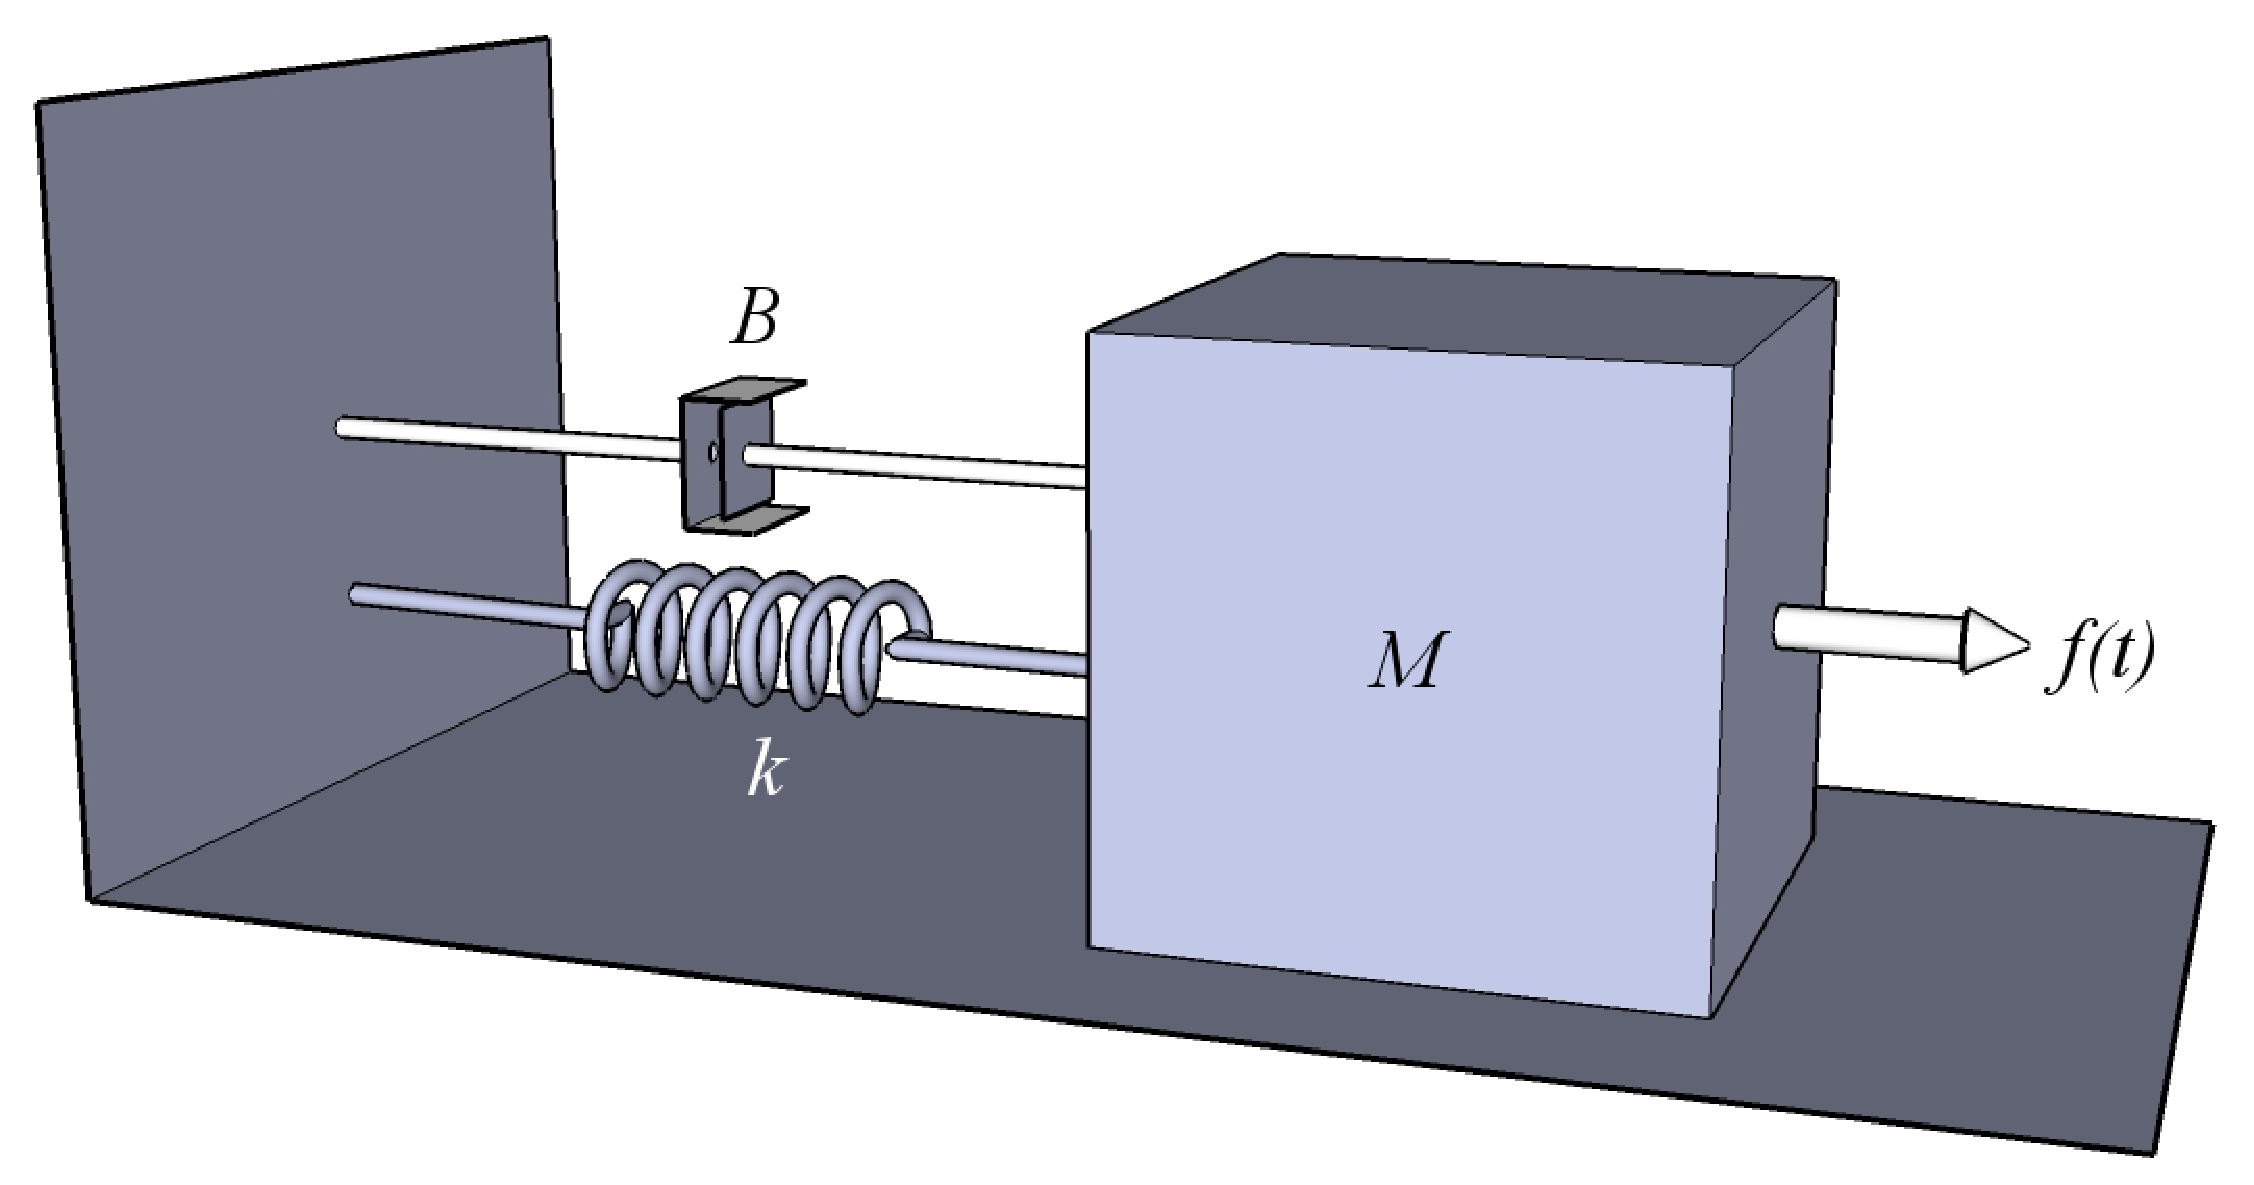
\includegraphics[width=.6\textwidth]{mechdiagram}}
    \sbox{\tempsmallA}{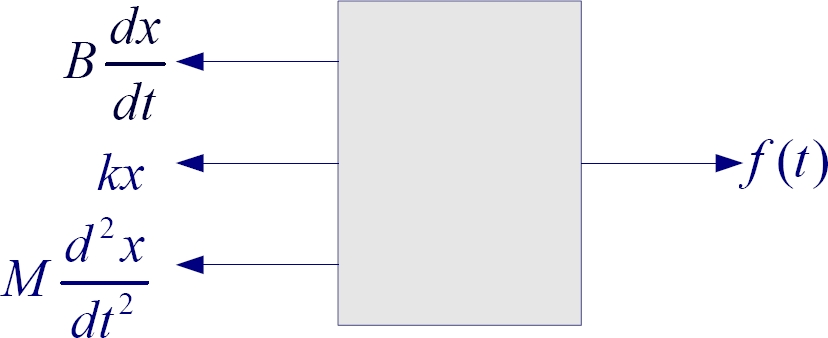
\includegraphics[width=.35\textwidth]{mechfreebody}}
    \newlength{\subfigoffsetA}
    \setlength{\subfigoffsetA}{0.5\ht\tempbigA}
    \addtolength{\subfigoffsetA}{-0.5\ht\tempsmallA}
    \subfloat[
            Mechanical translational system
            \label{fig.mechdiagram}
            ]{
            \usebox{\tempbigA}
            }
    \hfill
    \subfloat[
            Free-body diagram
            \label{fig.freebody}
            ]{
            \raisebox{\subfigoffsetA}{\usebox{\tempsmallA}}
            }
    \caption{}
\end{figure}

Applying Newton's Second Law, we have
\begin{equation}
    M\frac{d^2 x(t)}{dt^2} + B\frac{d x(t)}{dt} + kx = f(t)
        \label{eq.mechfreebody}
\end{equation}
The transfer function model is obtained by taking the Laplace transform (with zero initial conditions), which results in:
\begin{equation}
    G(s) = \frac{X(s)}{F(s)} = \frac{1}{Ms^2 + Bs + k}
        \label{eq.mechtf}
\end{equation}
You may note that for complicated mechanical systems, it is easier to draw the electric circuit force-voltage analogy in place of the free-body diagram.  In the force-voltage analogy, mass ($M$) is analogous to inductance, spring compliance ($1/K$) is analogous to capacitance, damping coefficient ($B$) is analogous to resistance, and velocity ($\dot{x}$) is analogous to current.  The key point in drawing the electric circuit analogy is to identify the displacement or velocity of each element and draw the circuit accordingly.  The circuit can be drawn in the s-domain to find the transfer function or in the time domain which is suitable for obtaining the state space model.  The electric circuit analogy for this mechanical system is shown in Figure~\ref{fig.mechelecanalogy}.

\begin{figure}[bht]
\centering
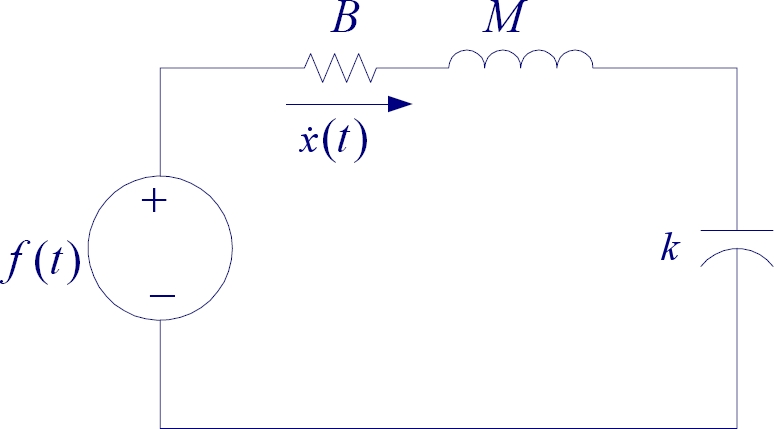
\includegraphics[width=.5\textwidth]{mechelecanalogy}
\caption{\footnotesize
        Electric circuit analogy for the mechanical system in Fig.\ \ref{fig.mechdiagram}
        \label{fig.mechelecanalogy}
        }
\end{figure}

With Kirchhoff's voltage law applied to the electric circuit, we get
\begin{equation}
    M\frac{d\dot{x}(t)}{dt} + B\dot{x}(t) + k\int_0^t \dot{x}(\sigma) = f(t)
\end{equation}
which is of course mathematically equivalent to (\ref{eq.mechfreebody}).  Equation~(\ref{eq.mechfreebody}) can also be written in state space form by selecting the two state variables as displacement and velocity: $x_1(t)=x(t)$ and $x_2(t) = \dot{x}(t)$.  The first-order differential equations then become
\begin{equation} \label{eq.mechdiff}
\begin{split}
    \frac{dx_1(t)}{dt} & = x_2(t) \\
    \frac{dx_2(t)}{dt} & = \frac{1}{M}f(t) - \frac{k}{M}x_1(t) - \frac{B}{M}x_2(t)
\end{split}
\end{equation}
For convenience, we will define multiple outputs: $y_1 = x_1(t)$ and $y_2 = x_2(t)$.  Thus the state space expression of this system is
\begin{equation}
\begin{split}
    \left[ \begin{array}{c} \dot{x}_1(t) \\ \dot{x}_2(t) \end{array} \right]
    & =
    \left[ \begin{array}{cc} 0 & 1 \\ -\frac{k}{M} & -\frac{B}{M} \end{array}
        \right]
    \left[ \begin{array}{c} x_1(t) \\ x_2(t) \end{array} \right]
    +
    \left[ \begin{array}{c} 0\\ \frac{1}{M} \end{array} \right]
    f(t)
    \\
    \left[ \begin{array}{c} y_1(t) \\ y_2(t) \end{array} \right]
    & =
    \left[ \begin{array}{cc} 1&0\\0&1 \end{array} \right]
    \left[ \begin{array}{c} x_1(t) \\ x_2(t) \end{array} \right]
\end{split}
\end{equation}
The simulation diagram for Equations~(\ref{eq.mechdiff}) is shown in Figure~\ref{fig.mechsimdiagram}

\begin{figure}[bht]
\centering
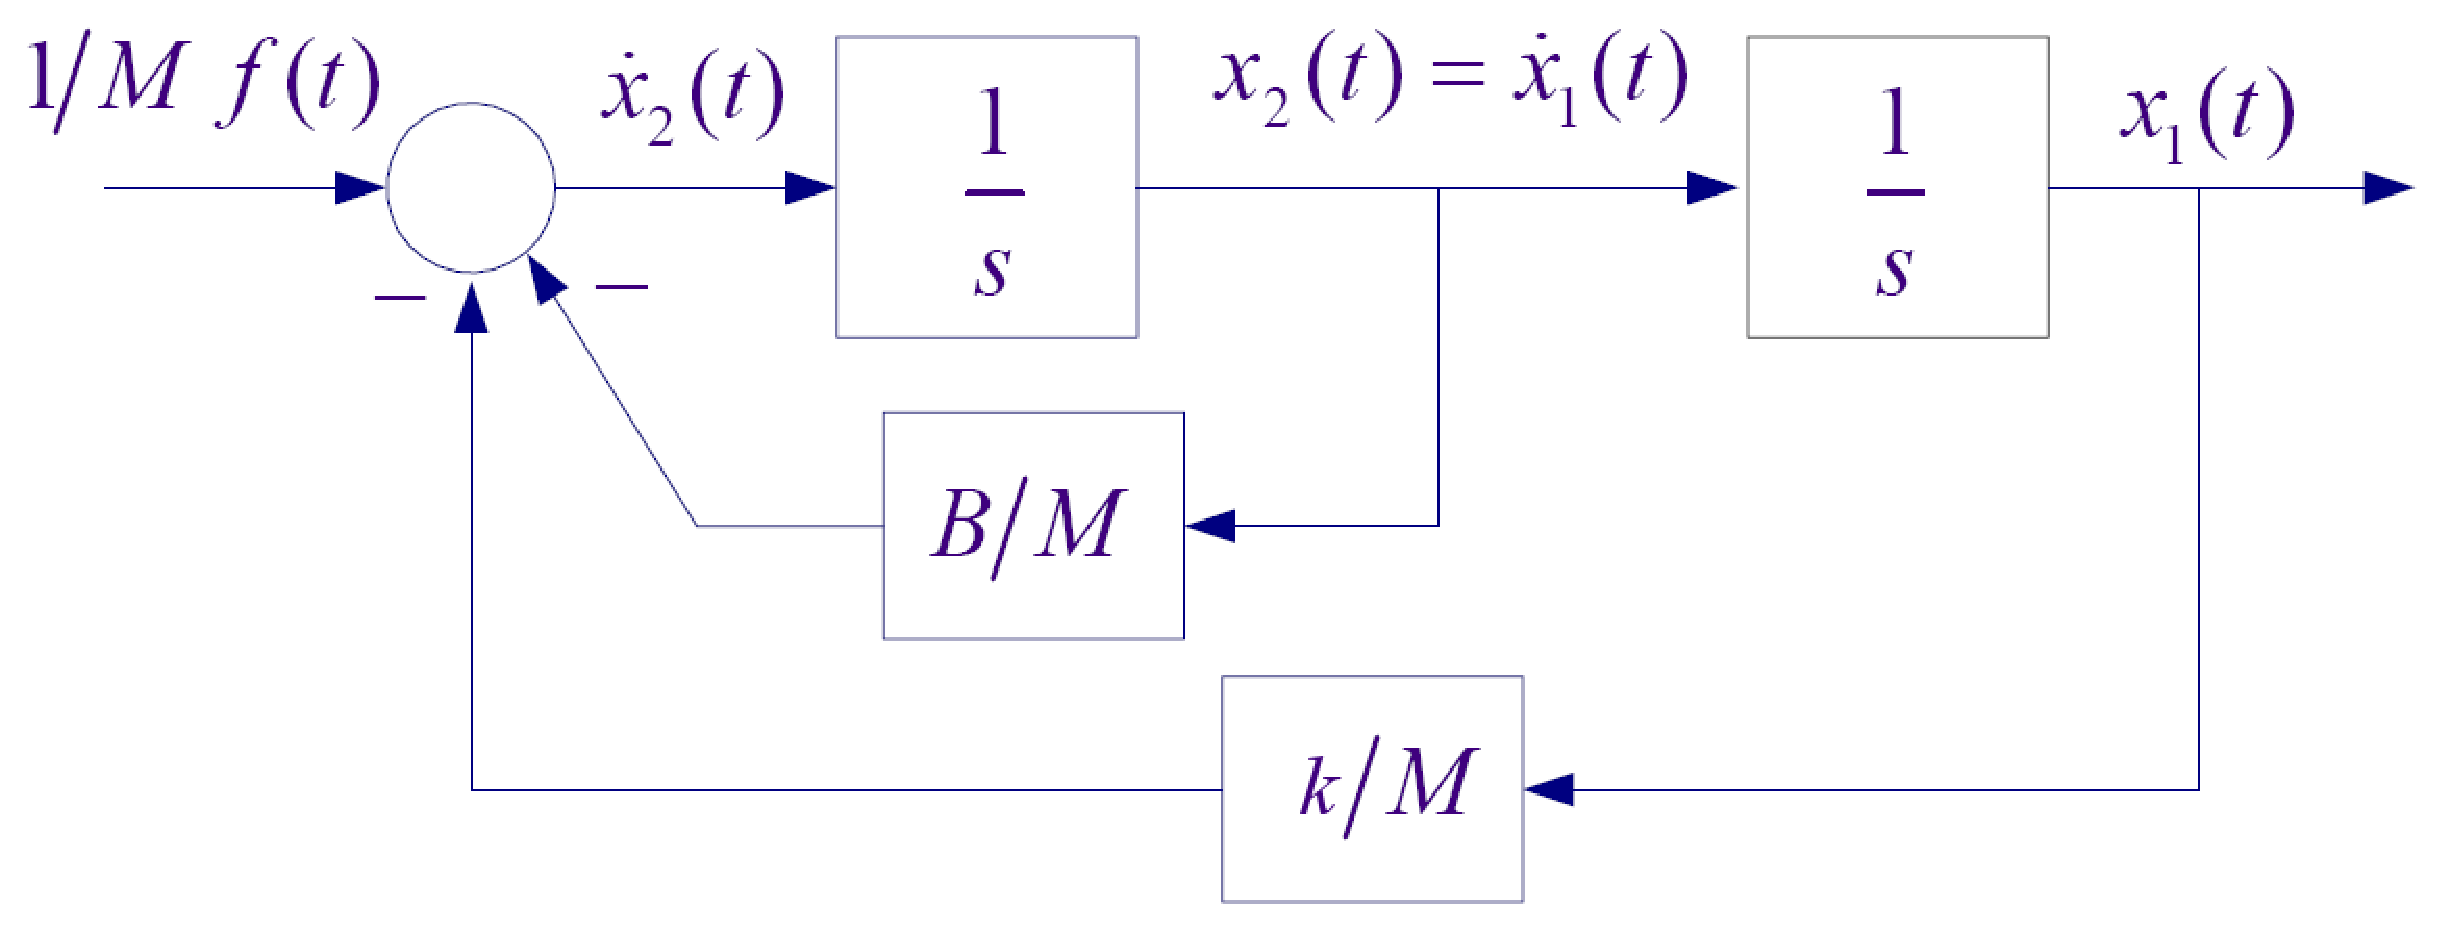
\includegraphics[width=.6\textwidth]{mechsimdiagram}
\caption{\footnotesize
        Simulation diagram for the mechanical system in Case Study~\ref{cs.mechtrans}
        \label{fig.mechsimdiagram}
        }
\end{figure}

With the system initially at rest, a constant force of $f(t) = 32$~Newtons is applied at time $t=0$.  The system in question has a mass of $2$~kg and a spring constant of $32\mbox{ kg}/\mbox{s}^2$.  We are told that the damping coefficient, $B$, may be adjusted to obtain a desirable response.
\par
The system's characteristic equation---from Eq.\ (\ref{eq.mechtf})---is given by
\begin{equation}
    s^2 + \frac{B}{M} s + \frac{k}{M} = 0
\end{equation}
which may be compared to the standard second-order transfer function
\begin{equation}
    s^2 + 2 \zeta \omega_n + \omega_n^2 = 0
\end{equation}

\subsubsection{Pre-lab Exercises}
\begin{enumerate}
\item
    The dashpot damping is adjusted to $B = 2\mbox{ Ns/m}$.  Determine the natural frequency of oscillation ($\omega_n$), damping ratio ($\zeta$), percent overshoot ($PO = 100e^{-\frac{\zeta\pi}{\sqrt{1-\zeta^2}}}$), peak time ($t_p = \frac{\pi}{\omega_n \sqrt{1-\zeta^2}}$), and settling time ($t_s \approx 4\tau$).
\item
    The dashpot damping is adjusted to $B = 56\mbox{ Ns/m}$.  Determine the damping ratio, $\zeta$, response time constants $\tau_1$ and $\tau_2$, and settling time $t_s \approx 4\max\left(\tau_1,\tau_2\right)$.
\item
    Determine the friction coefficient $B$ for the response to be critically damped.  What is the response time constant and approximate settling time?
\end{enumerate}

\subsubsection{Lab Exercises (Digital Simulation using Simulink)}
To create a Simulink block diagram representation of the system shown in Figure~\ref{fig.mechsimdiagram} double click on the Simulink icon on the MATLAB toolbar.An untitled window for designing
and simulating a new model will open. Double click on the Simulink library icon, this will open
nine subsystems libraries. Open the Source Library and drag the Step Input block to the open new
model window. Double click on the Step Input to open its dialog box, set the parameters Step time
to 0, and Final value to 32. Get two integrators from the Continuous library, three Gain blocks
on one Sum block from the Math Library, one Scope and one XY Graph from the Sink library,
one Mux block from Signals and Systems library. Open the Sum block dialog box and enter the
required summing point signs + - -. Once you have dragged all the required blocks and placed
them on the new model window, join the in-ports and out-ports to create the simulation model.
The purpose of Mux block (Multiplex) is to combine the velocity and displacement signals into a
composite signal so as to display both signals on one Scope. XYGraph is used to display the state
trajectory, i.e., velocity versus displacement plot. Connect $x_1$ to the first input and $x_2$ to the second
input of the XY Graph. Open the XY Graph dialog box, set the $x$-axis limits to 0, 2, the $y$-axis
limits to $\pm4$ and Sample time to $0.01$. An mfile named \texttt{MSFanimation.m} has been developed for
animating the motion of the mass-spring-friction system during simulation. To add this animation,
get an S-Function block form the functions \& Tables library, place it on your model window and
connect its input terminal to the signal coming from the output of the Mux block. Make sure that
you have obtained \texttt{MSFanimation.m} and \texttt{InAmin.m} files from your instructor and placed it on a
folder in the current directory. Open the S-Function block for its name enter \texttt{MSFanimation}, and
for the S-Function parameter enter $0.01$.
Set the gain blocks to the given values and the damping coefficient specified part 1 of the Pre-lab exercises.
\par
Before starting simulation, you must set the simulation parameters.  Pull down the Simulation dialog box and select Simulation Parameters.  Set the start time to 0 and the stop time to a suitable value.  For the Solver option, select Variable-step and any of the Continuous integration routines such as \texttt{ode45} or \texttt{ode23}.  For more accurate step response you may change the Relative tolerance from $10^{-3}$ to $10^{-5}$.  If you select Fixed-step, again make sure you select a Continuous integration routine such as \texttt{ode4} (Runge-Kutta).  You can also change the step size from auto to a small value such as $0.0001$.  Follow the same procedure in the remaining case studies in this lab and make sure the Solver option is \textit{not} set to Discrete.
\par
Simulate and obtain a print of the Scope.  The scope yellow trace will not print well.  Also, the Simulink XY Graph cannot be printed.  A script m-file named \texttt{plotscope.m} has been developed which captures the scope plot and produces a Figure plot.  At the MATLAB prompt, type \texttt{plotscope} and then click on the Scope Figure (outside the plot area) and hit return.  You can add labels and a legend or edit the graph.  You can use this procedure for the XY Graph or the animation plot.
\par
An alternative way to obtain a Figure plot is to place two To Workspace blocks from the Sink library and connect their inputs to the  $x_1$ and $x_2$ signals and defining \texttt{x1} and \texttt{x2} for the variables.  The time array can be obtained by feeding a Clock block into another To Workspace block and defining a variable \texttt{t} for time. After performing the simulation you can use the \texttt{plot} function to obtain the desired Figure plot.
\par
Repeat the simulation for the value of $B$ in questions 2 and 3 in the Pre-lab.  Document the plots obtained for the above three cases, determine and summarize the time-domain specifications for each case.  Comment on the nature of each response and discuss the effect of damping coefficient on the resulting response.

\begin{figure}[bht]
\centering
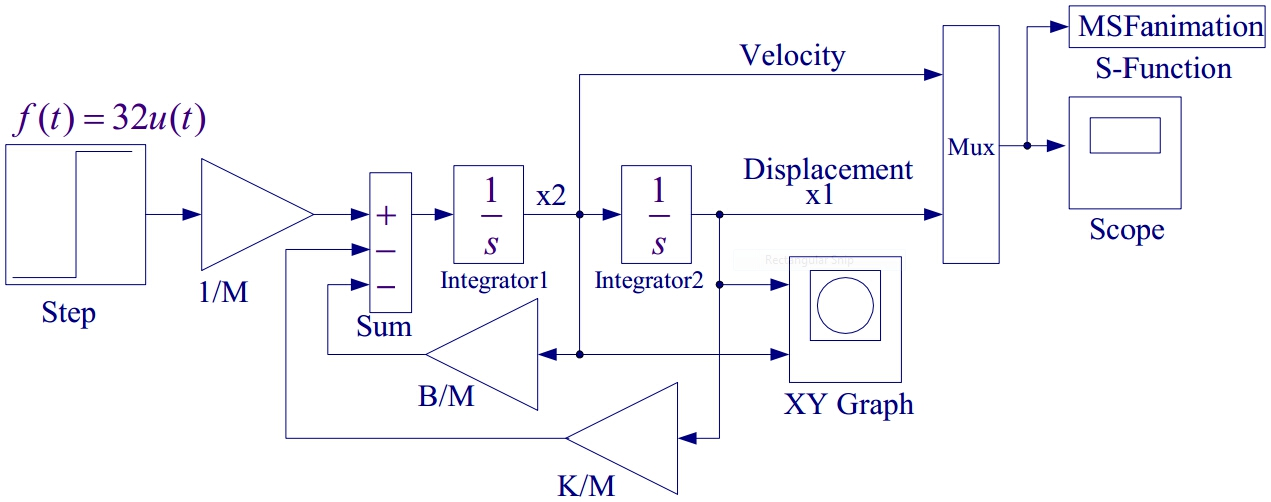
\includegraphics[width=.9\textwidth]{MechTransSimulink}
\caption{\footnotesize
        Simulink diagram for the mechanical system in Case Study 1.
        \label{fig.mechsimulink}
        }
\end{figure}

\subsection{Case Study 2: Simple Pendulum}
\label{cs.simplepend}

\begin{figure}[thb]
\centering
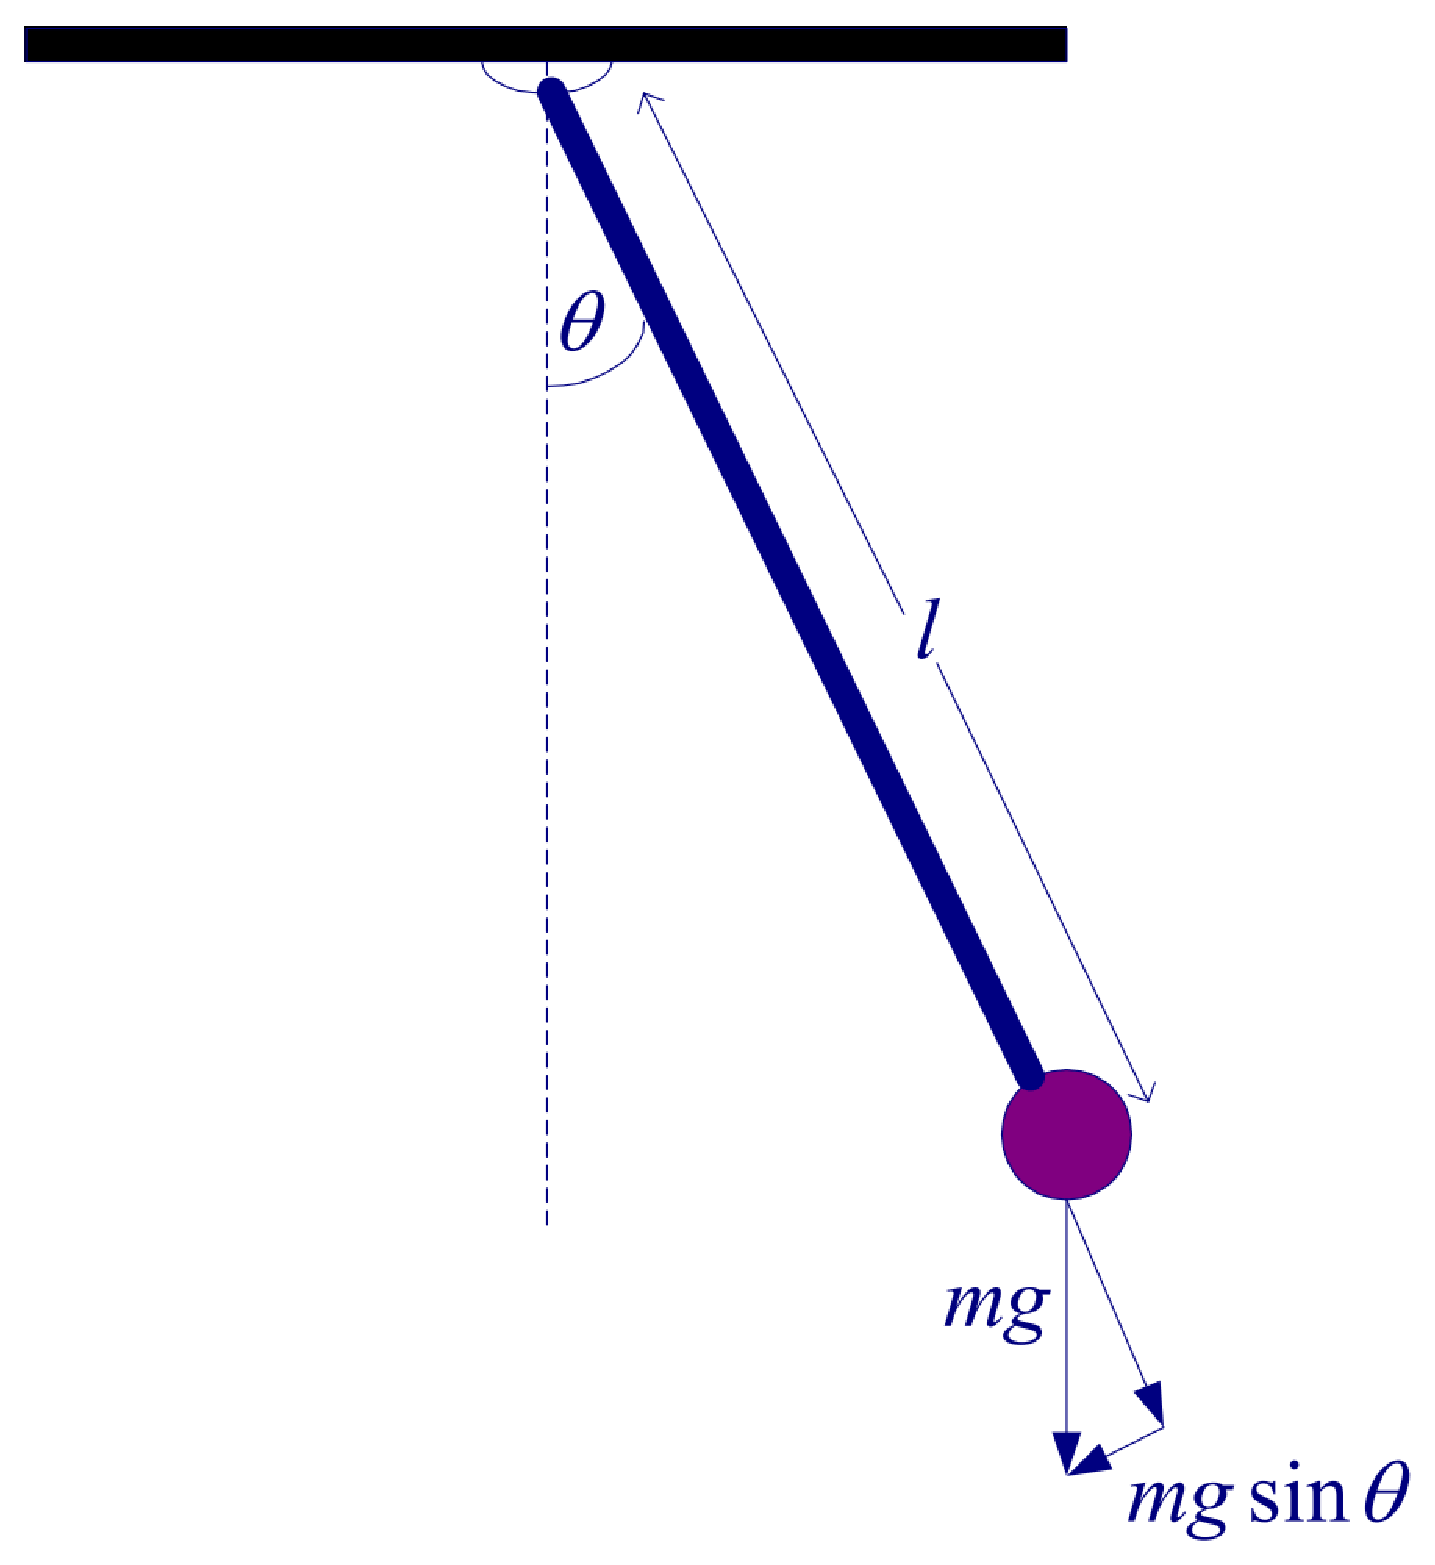
\includegraphics[width=.4\textwidth]{PendModel}
\caption{\footnotesize
        Simple pendulum.
        \label{fig.penddiagram}
        }
\end{figure}

Consider the simple pendulum illustrated in Figure~\ref{fig.penddiagram} where a mass of $m$ kg hangs from a hinge by a rod of length $l$ meters.  The rod is light enough that its mass can be neglected.  The rod is displaced by angle $\theta$ radians from the equilibrium position.  Assume a viscous friction for the motion with a damping coefficient of $B$ kgs/m.  The tangential velocity of the mass is $l\dot{\theta}$.  The tangential forces acting to restore the pendulum to equilibrium are
\begin{equation}
    F_T = -mg\sin(\theta) - Bl\dot{\theta}
\end{equation}
where $g$ is the gravitational acceleration.  Also from Newton's law, we have
\begin{equation}
    F_T = ml\ddot{\theta}.
\end{equation}
Combining the above equations, we get
\begin{equation}    \label{eq.nonlinearpend}
    \ddot{\theta} + \frac{B}{m}\dot{\theta}+\frac{g}{l}\sin(\theta) = 0.
\end{equation}
Equation~\eqref{eq.nonlinearpend} is nonlinear because of the $\sin(\theta)$ term.  We can now write the above equation in state variable form.  Let $x_1 = \theta$ and $x_2 = \dot{\theta}$ (angular velocity).  Then,
\begin{subequations}    \label{eq.pendstates}
    \begin{flalign}
        \dot{x}_1 &= x_2 \\
        \dot{x}_2 &= -\frac{B}{m}x_2-\frac{g}{l}\sin(x_1).
    \end{flalign}
\end{subequations}
\par
The simulation diagram for equations~\eqref{eq.pendstates} is shown in Figure~\ref{fig.pendstatediagram}.  The mass is displaced from the equilibrium by $0.5$ radians (28.65\textdegree) at time $t=0$.  The mass is $0.5\mbox{ kg}$, the rod length is $0.613\mbox{ m}$, and the gravitational acceleration is $9.81\mbox{ m/s}^2$.  Two cases of frictional coefficient will be considered:
\begin{enumerate}
\item
    $B = 0.05$ kgs/m
\item
    $B = 4.0$ kgs/m
\end{enumerate}

\begin{figure}[thb]
\centering
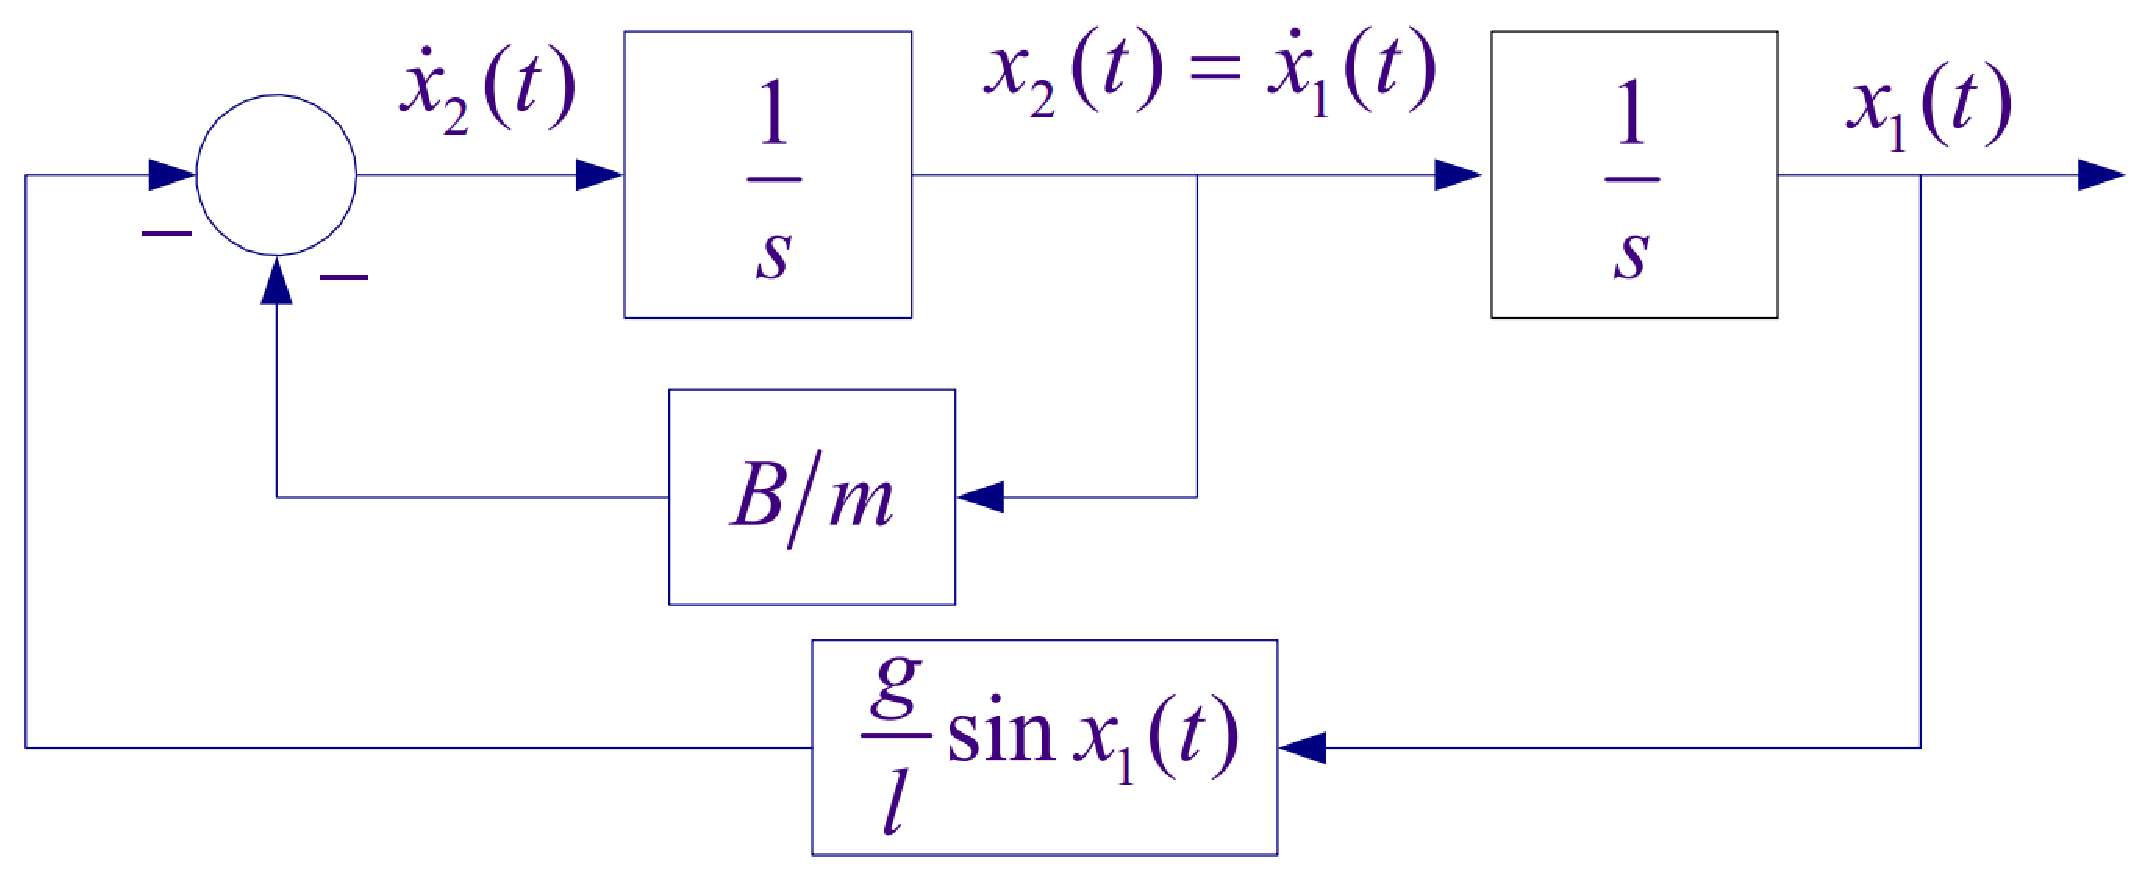
\includegraphics[width=.6\textwidth]{PendSysDiagram}
\caption{\footnotesize
        Simple pendulum.
        \label{fig.pendstatediagram}
        }
\end{figure}

\subsubsection{Lab Exercises (Digital Simulation using Simulink)}

Create a Simulink block diagram presentation of the system shown in Figure~\ref{fig.penddiagram}.  Drag all the required blocks and place them on a new model window.  For the nonlinear term, get the \texttt{Fcn} block from the Function \& Tables library.  Use \texttt{u} for the input variable name, e.g.\ $16*\sin(u)$.  Specify the gain $B/m$ and connect all blocks to create the simulation model shown in Figure~\ref{fig.pendsimulink}.
\par
Open the last integrator dialog box and set the initial condition to $0.5$ for the angular displacement.  The initial velocity is zero.  Therefore, set the initial condition parameter for the first integrator to 0.  Place one scope to display the angle $\theta$ (signal $x_1$) and another scope to display the velocity signal $x_2$. Use an XY Graph to display the state trajectory, i.e., velocity versus displacement plot.  Connect $x_1$ to the first input and $x_2$ to the second input.  Open the XY Graph dialog box, and set the $x$-axis limits to $-5,0.5$, the $y$-axis limits to $\pm2$, and the sample time to $0.01$.

\begin{figure}[thb]
\centering
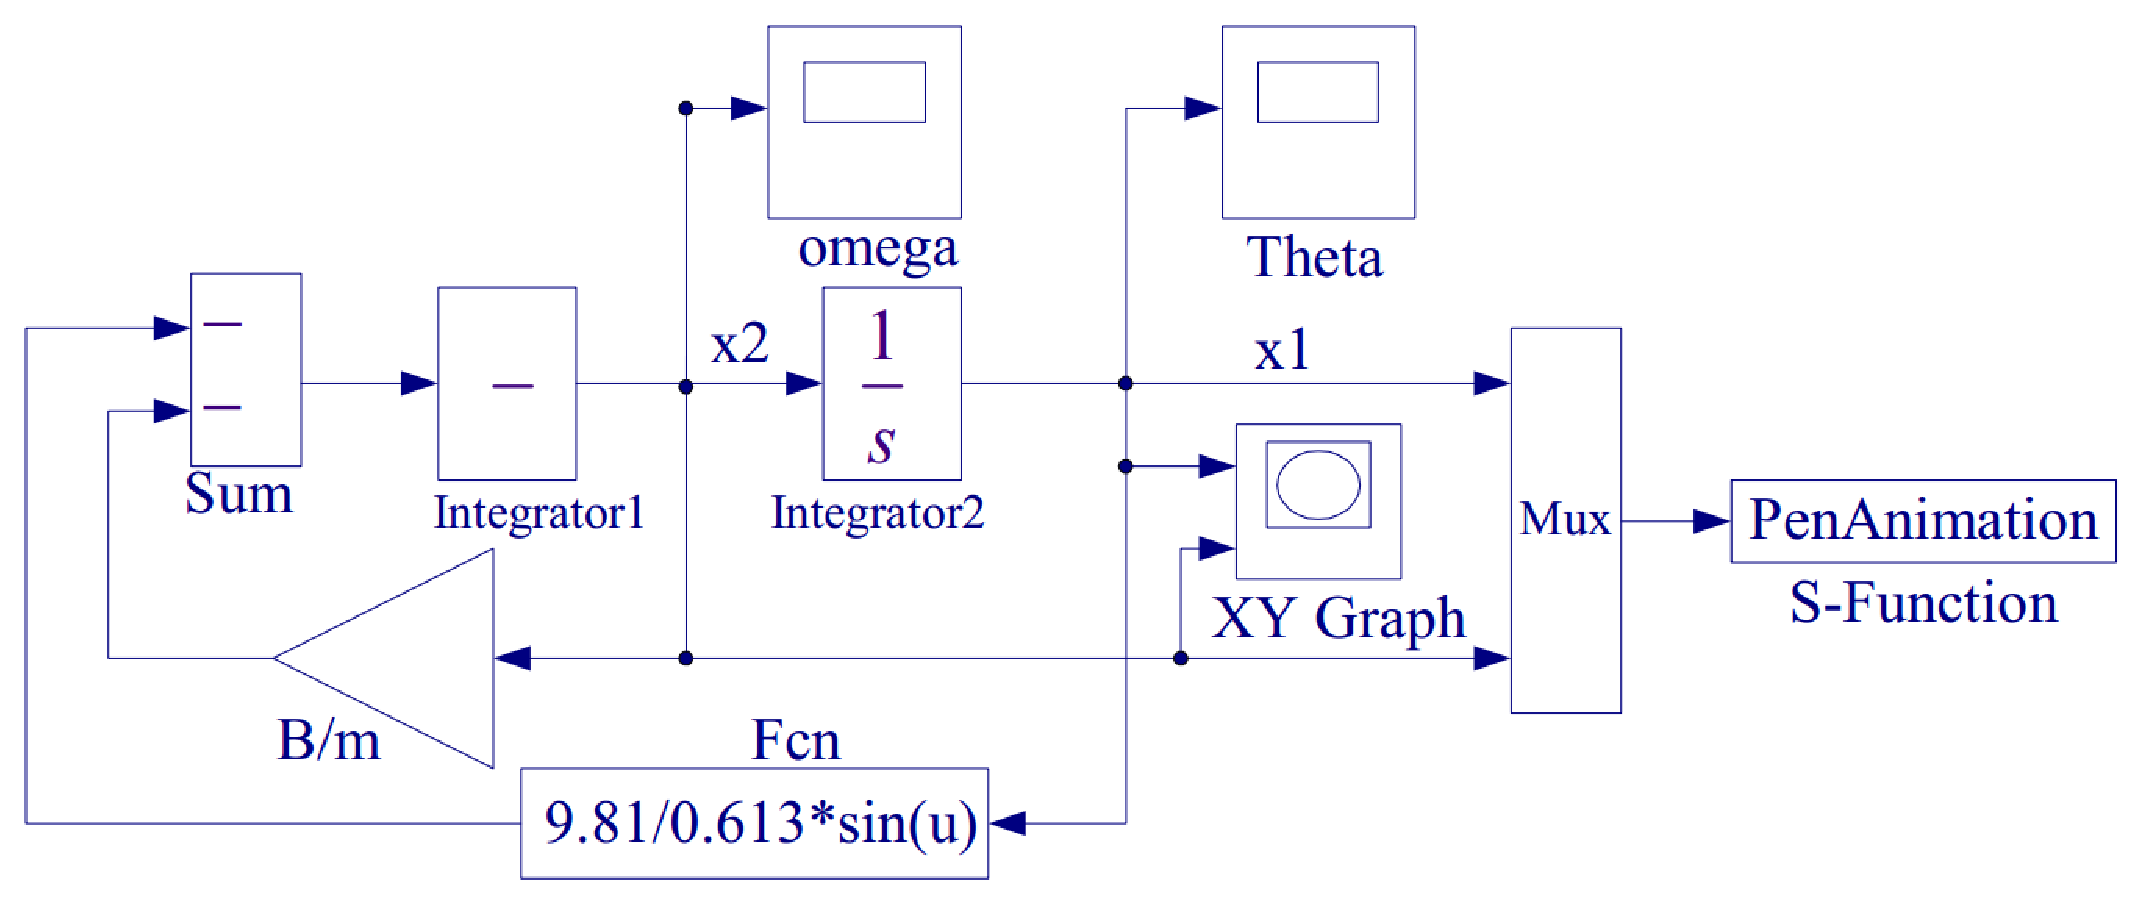
\includegraphics[width=.9\textwidth]{PendSimulink}
\caption{\footnotesize
        Simulink diagram for the pendulum in Case Study 2.
        \label{fig.pendsimulink}
        }
\end{figure}

\par
An m-file named \texttt{PenAnimation.m} has been developed for animating the pendulum swing during simulation.  To add this animation, get a Mux block with two inputs.  Connect $x_1$ to the top in-port and $x_2$ to the lower in-port.  Next get an S-Function block from the Functions \& Tables library, place it on your model window and connect its in-port terminal to the signal coming from the Mux block.  Make sure that you have obtained this m-file from your instructor and placed it on a folder in the path of MATLAB.  Open the S-Function block, for its name enter \texttt{PenAnimation} and for the S-Function parameter, enter $0.01$.

\begin{enumerate}
\item
    Set the friction coefficient to $0.05\mbox{ kgs/m}$.\\
    Simulate and print the zero-input response (natural response) for the angular displacement and state trajectory.  You may want to reduce the simulation final time to a suitable value.  Comment on the nature of the response.  When a system returns to its equilibrium point after a disturbance, the system is said to be \textit{stable}.  Is the system stable about its equilibrium point $\theta=0$?  How would you describe the system stability if the damping coefficient $B$ were neglected?  Use \texttt{plotscope} to capture the Scope trace and XY Graph.
\item
    Repeat the above for $B=4\mbox{ kgs/m}$.
\end{enumerate}

\subsubsection{Linearization}

Many control systems are designed to return to their equilibrium position when subjected to a small disturbance.  Nonlinear systems are often \textit{linearized} assuming small deviation from the equilibrium point.  The nonlinear differential equation describing the motion of the pendulum can be linearized if the initial angle of deflection is small.
\par
Let $\theta = \theta_0+\Delta\theta$ and substitute this $\theta$ into~\eqref{eq.nonlinearpend} and expand the sine term.  For small $\Delta\theta$, we assume that $\sin(\Delta\theta)\approx\Delta\theta$, $\cos(\Delta\theta)\approx 1$, and $\cos(\theta_0)\approx 1$.  Show that~\eqref{eq.nonlinearpend} results in the linearized differential equation
\begin{equation}    \label{eq.linearizedpend}
    \frac{d^2\Delta\theta}{dt^2} + \frac{B}{m}\frac{d\Delta\theta}{dt} + \frac{g}{l}\frac{d\Delta\theta}{dt}.
\end{equation}
This approximation is reasonably accurate for $-\pi/4\leq\theta\leq\pi/4$.

\begin{enumerate}
\setcounter{enumi}{2}
\item
    The state variable in terms of the small changes $\Delta\theta$ and $\frac{d\Delta\theta}{dt}$ is the same as in~\eqref{eq.pendstates}, except $\sin x_1$ is replaced by $x_1$.  Copy the Simulink nonlinear model and paste it on the same model window, replace the \texttt{Fnc} block with a gain bloc and set the parameter to the value given by $g/l$. Eliminate the S-function in the duplicate model.  In order to validate the linearized model use a Mux block with two inputs and connect the in-ports to the $x_1$ signal of each model and a Scope to its out-port terminal.  Simulate for $B=0.05$ in both models and obtain the response.  State if the linearized model response is in close agreement with the nonlinear model.  The characteristic equation of the linearized model is
    \begin{equation}
        s^2 + \frac{B}{m}s + \frac{g}{l} = 0.
    \end{equation}
\item
    For the given values of $l$ and $m$, find the value of $B$ for critically damped response.  Set the $B$ to this value in both models and repeat the simulation.  Comment on the response.
\end{enumerate}

\subsection{Case Study 3: Nonlinear Differential Equation with Saturation}
\label{cs.saturation}
One of the useful features of Simulink is the availability of nonlinear blocks such as \texttt{switch}, \texttt{relay}, \texttt{deadzone}, \texttt{backlash}, \texttt{rate-limiter}, \texttt{saturation}, \texttt{Coulomb friction}, and many other nonlinear functions.  These are very useful for studying effects of nonlinearities on the behavior of the system.  This study deals with the simulation of a nonlinear differential equation.  The angular displacement of a dynamic system is given by
\begin{equation}    \label{eq.deltasat}
    \ddot{\delta} + 4\dot{\delta} + a_0\sin(\delta) = 30u(t)
\end{equation}
where $u(t)$ is a unit step, $\delta$ is constrained to be between $\pm 2\pi$, and
\begin{equation}    \label{eq.aswitch}
    a_0 = \begin{cases}35.6, & 0\leq t\leq t_c \\ 15, & t_c < t < \infty \end{cases}
\end{equation}
where $t_c$ is a threshold switching time.  Large values of $t_c$ may result in an unbounded response.  Transforming to state variable form, let $x_1 = \delta$ and $x_2 = \dot{\delta}$.  Then
\begin{subequations}
    \begin{flalign}
        \dot{x_1} &= x_2\\
        \dot{x_2} &= -a_0\sin x_1 -4x_2 + 30u(t).
    \end{flalign}
\end{subequations}

The Simulink diagram for the above system is shown in Figure~\ref{fig.satsimulink}.  Equation~\eqref{eq.aswitch} is represented by the \texttt{switch} block and \eqref{eq.deltasat} is represented by the \texttt{saturation} block.

\begin{figure}[thb]
\centering
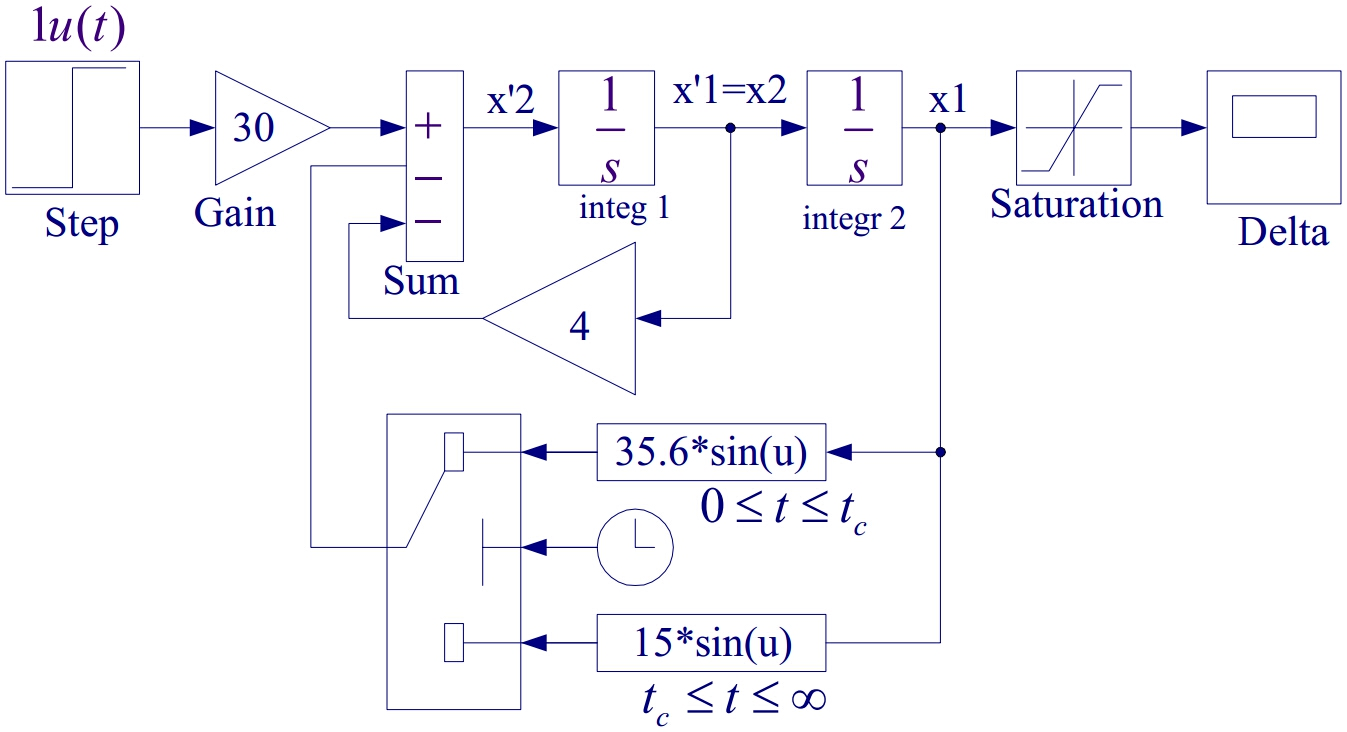
\includegraphics[width=.6\textwidth]{SatSimulink}
\caption{\footnotesize
        Simulink diagram for Case Study 3.
        \label{fig.satsimulink}
        }
\end{figure}

\subsubsection{Lab Exercises (Digital Simulation using Simulink)}
Construct the Simulink diagram as in Figure~\ref{fig.satsimulink}.  In the \texttt{step} block, set the step time to 0 and the final time to 1. \par
Open the Simulation Parameters dialog box.  Set the stop time to 5 seconds and select \texttt{ode45}.  Obtain the response for $t_c=0.4$ and $t_c = 3$.  Comment on the behavior of the response for each case.

\subsection{Case Study 4: Inverted Pendulum}
This fourth study deals with the classic problem of balancing an inverted pendulum. This study
demonstrates the control of an inherently unstable system of balancing systems that occurs in the
areas of missile stabilization and robotics. This study also demonstrates the linearization of a
nonlinear system.

\begin{figure}[thb]
\centering
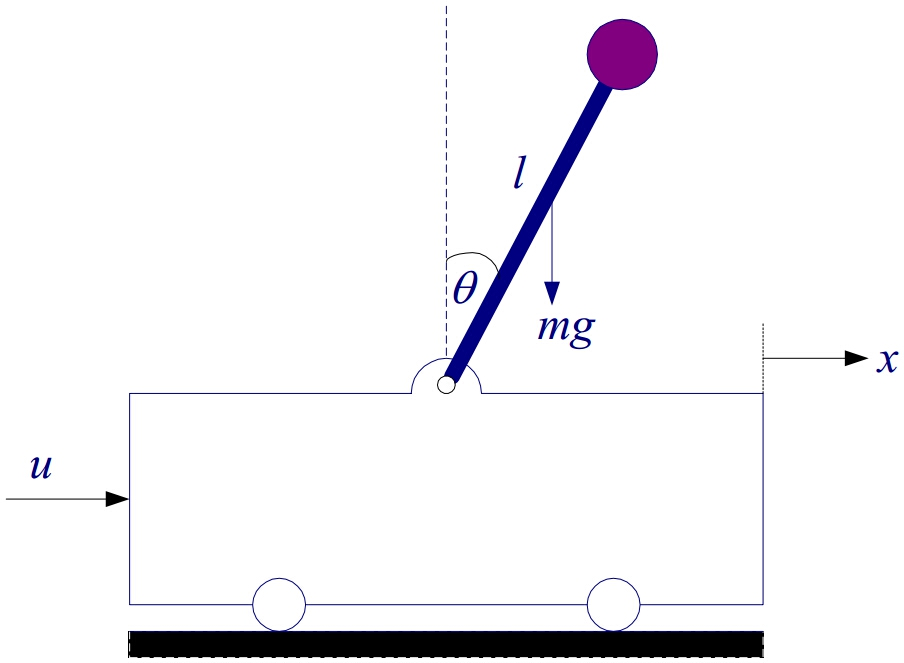
\includegraphics[width=.6\textwidth]{InvPendDiagram}
\caption{\footnotesize
        Simulink diagram for Case Study 3.
        \label{fig.invpenddiagram}
        }
\end{figure}

Figure~\ref{fig.invpenddiagram} shows an inverted pendulum of length $l$ and mass $m$ supported by a frictionless pivot on a cart of mass $M$.  It is to be balanced be means of a force $u$ applied to the cart.  That is, the cart must be moved in such a way that the pendulum is in the upright position.  In a physical system there would be sensors to measure the position and velocity of the cart and angle $\theta$ measured from the vertical position.  This is also a model of the attitude control of a space booster on takeoff.  This is similar to balancing a broomstick on the palm of your hand.  The equilibrium condition is when $\theta(t)$ and $\dot{\theta}(t)$ return to zero.  The visual location of your hand and the position of the broomstick and the proper movement of your hand is the required feedback without which it is not possible to balance the broomstick.  The differential equations describing the motion of the system by summing the forces on the pendulum result in the following nonlinear equations:
\begin{subequations}    \label{eq.invpendnonlineardiffeq}
    \begin{gather}
        (M+m)\ddot{x} + (mL\cos\theta)\ddot{\theta} = (mL\sin\theta)(\dot{\theta})^2 + u \\
        (mL\cos\theta)\ddot{x} + mL^2\ddot{\theta} = mgL\sin\theta .
    \end{gather}
\end{subequations}

\subsubsection{Pre-Lab Exercise}
Linearize equations~\eqref{eq.invpendnonlineardiffeq} in the neighborhood of the zero initial states.  \textit{Hint: Substitute $\theta$  for $\sin\theta$, 1 for $\cos\theta$ and $0 for (\dot{\theta})^2$.}  With the state variables defined as $x_1 = \theta$, $x_2 = \dot{\theta}$, $x_3 = x$, and $x_4 = \dot{x}$, show that the linearized state equation is
\begin{equation}
    \left[\begin{array}{c}
        \dot{x}_1\\
        \dot{x}_2\\
        \dot{x}_3\\
        \dot{x}_4
    \end{array}\right]
    =
    \left[\begin{array}{cccc}
        0   &   1   &   0   &   0   \\
        \frac{M+m}{ML}g&0&0 &   0   \\
        0   &   0   &   0   &   1   \\
        \frac{-m}{M}g&0&0   &   0
    \end{array}\right]
    \left[\begin{array}{c}
        x_1\\
        x_2\\
        x_3\\
        x_4
    \end{array}\right]
    +
    \left[\begin{array}{c}
        0\\
        \frac{-1}{ML}\\
        0\\
        \frac{1}{M}
    \end{array}\right]
    u.
\end{equation}
If we want to have all the state variables available as output, we define the $C$ matrix as the identity and $D$ as a $4\times1$ zero matrix.

\subsubsection{Lab Exercises (Digital Simulation using Simulink)}
The parameters of the inverted pendulum are $M=4\mbox{ kg}$, $m=0.2\mbox{ kg}$, $L = 0.5\mbox{ m}$, and $g = 9.81\mbox{ m/s}^2$.  Let the initial state vector be
\begin{equation}
    x_0 = \left[\begin{array}{c}
        0.1\\0\\0.1\\0
        \end{array}\right].
\end{equation}
In a MATLAB script file, define the system parameters and the $A,B,C,D$ matrices.
\par
Save the file as \texttt{Lab4CS4aData.m}.
\par
Launch Simulink, open a new model, get the \texttt{State-Space} block from the Continuous library, and construct the above state model.  Double click on the \texttt{State-Space} block to open its dialog box and for the parameters type \texttt{A}, \texttt{B}, \texttt{C}, and \texttt{D}.  Note that MATLAB is case-sensitive.  For the initial condition, type \texttt{x0} (or however you defined the initial conditions in your script).  In the Simulation Parameters dialog box set the Start time to 0 and the Stop time to 3.  For the Solver option, use a variable step size and \texttt{ode45} algorithm.
\par
Connect a \texttt{Demux} block to separate the signals, and use two scopes to display $\theta$ and $x$.  Get an \texttt{Inport} block from the Source library and use it as an input terminal.  Also get an \texttt{Outport} block from the Sink library and connect it to the signal for $\theta$ as shown in Figure~\ref{fig.invpendsimulink}.

\begin{figure}[bht]
\centering
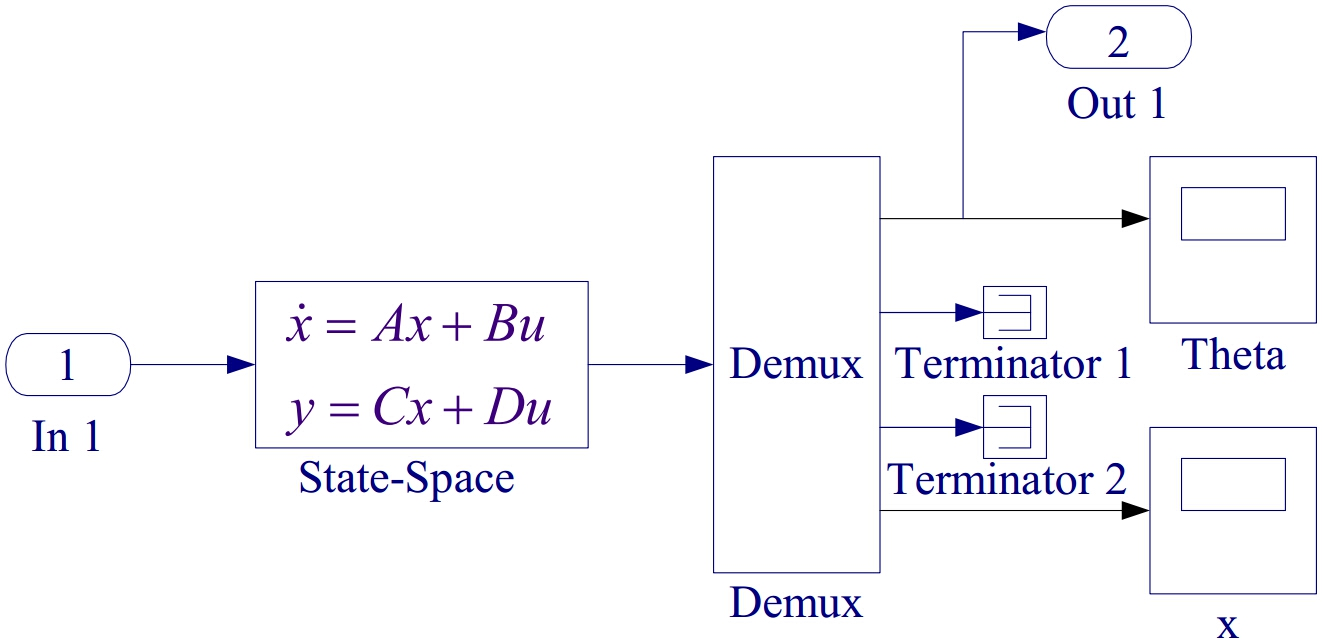
\includegraphics[width=.6\textwidth]{InvPendSimulink}
\caption{\footnotesize
        Simulink diagram for the inverted pendulum in Case Study 4.
        \label{fig.invpendsimulink}
        }
\end{figure}

Save the Simulink model as \texttt{Lab4CS4a.mdl}.
\par
Run the script m-file \texttt{Lab4CS4aData} at the MATLAB prompt to calculate the $A$, $B$, $C$, and $D$ matrices.  These values are now defined and are available in Simulink.  Start the simulation in Simulink and obtain a plot of $\theta$ and $x$.  Comment on the stability of the system.  MATLAB provides the function \texttt{linmod} to extract a linear model in state variables or as a transfer function model using the Simulink file name as an argument.  At the MATLAB prompt type the following commands to obtain the linearized transfer function model and roots of the characteristic equation:

\begin{codex}
[num, den] = linmod('Lab4CS4a');
r = roots(den);
\end{codex}

You may have found that the angle $\theta$ increases without limit, i.e. the response is unbounded.  Also you may find that a root of the characteristic equation is positive.  This again confirms an unbounded response and we say that the system is unstable, that is, the inverted pendulum will fall over unless a suitable control force via state feedback is used.
\par
The purpose is to design a control system such that for a small initial disturbance the pendulum can be brought back to the vertical position ($\theta = 0$), and the cart can be brought back to the reference position ($x=0$).
\par
One approach in modern control systems, accomplished by the use of state feedback, is known as \textit{pole-placement design}.  The pole-placement method allows all roots of the system characteristic equation to be placed in the desired locations.  This results in a regulator with a constant gain vector $K$.  In pole-placement design the control is achieved by feeding back the state variables through a regulator with constant gains.  Consider the control system presented in state-variable form:
\begin{subequations}    \label{eq.statespace}
    \begin{flalign}
        \dot{x}(t) &= Ax(t) + Bu(t) \\
        y(t)        &= Cx(t).
    \end{flalign}
\end{subequations}
Consider the block diagram of the system shown in Figure~\ref{fig.poleplacesys} with state feedback control
\begin{equation}    \label{eq.statefeedback}
    u(t) = -Kx(t),
\end{equation}
where $K$ is a $k\times 1$ matrix of constant feedback gain.  The control system input is assumed
to be zero. The purpose of this system is to return all state variables to values of zero when
the states have been perturbed.

\begin{figure}[bht]
\centering
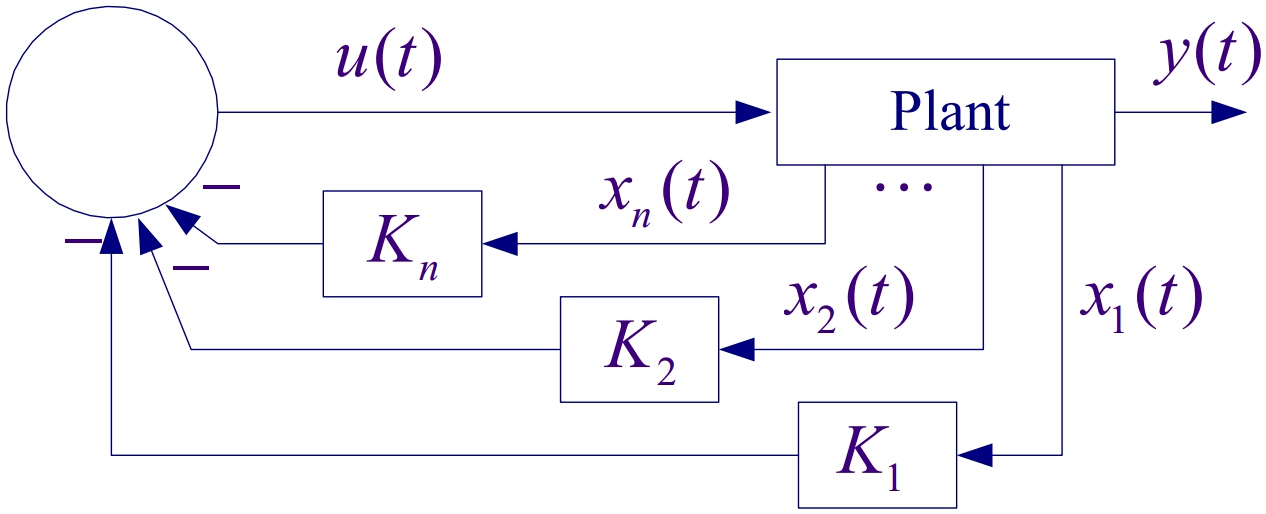
\includegraphics[width=.6\textwidth]{StateFeedbackSystem}
\caption{\footnotesize
        Control system design via pole-placement.
        \label{fig.poleplacesys}
        }
\end{figure}

Substituting \eqref{eq.statefeedback} into \eqref{eq.statespace}, the closed-loop system variable representation is
\begin{equation}
    \dot{x}(t) = [A-BK]x(t) = A_f x(t).
\end{equation}
The design objective is to find the gain matrix $K$ such that the characteristic equation for the controlled system is identical to the desired characteristic equation.  A custom-made function named \texttt{placepole} is developed for the pole placement design.  The syntax is
\begin{codex}
[K, Af] = placepole(A, B, C, P)
\end{codex}
where $A$, $B$, and $C$ are system matrices and $P$ is a row vector containing the desired closed-loop poles.  This function returns the gain vector $K$ and the closed-loop system matrix $A_f$.  Also, the MATLAB Control System Toolbox contains two function for pole-placement design (\texttt{acker} and \texttt{place}).
\par
An aspect of state variable design is state feedback design.  In this study we use the custom function \texttt{placepole} and design a state feedback controller to place the closed-loop poles at
\begin{equation*}
    P = \{-1\pm 0.5j, -4, -5\}.
\end{equation*}
\par
In your \texttt{Lab4CS4aData4.m} script, append a definition of $P$ and use it to call \texttt{placepole}.
\par
In Simulink, open \texttt{Lab4CS4a.mdl}.  Add the state feedbacks and set the gains to $K(1)$, $K(2)$, $K(3)$, and $K(4)$ as shown in Figure~\ref{fig.poleplacesimulink} and save the model as \texttt{Lab4CS4b.mdl}.  Run the script file to evaluate $K$ for use in Simulink.  Then state the simulation in Simulink and obtain a plot of $\theta$ and $x$.  Comment on the stability of the system.  To see an inverted  pendulum animation, make sure you have obtained the m-file named \texttt{InvPenAnimation.m}.  After simulation, type \texttt{InvPenAnimation} at the MATLAB prompt.

\begin{figure}[bht]
\centering
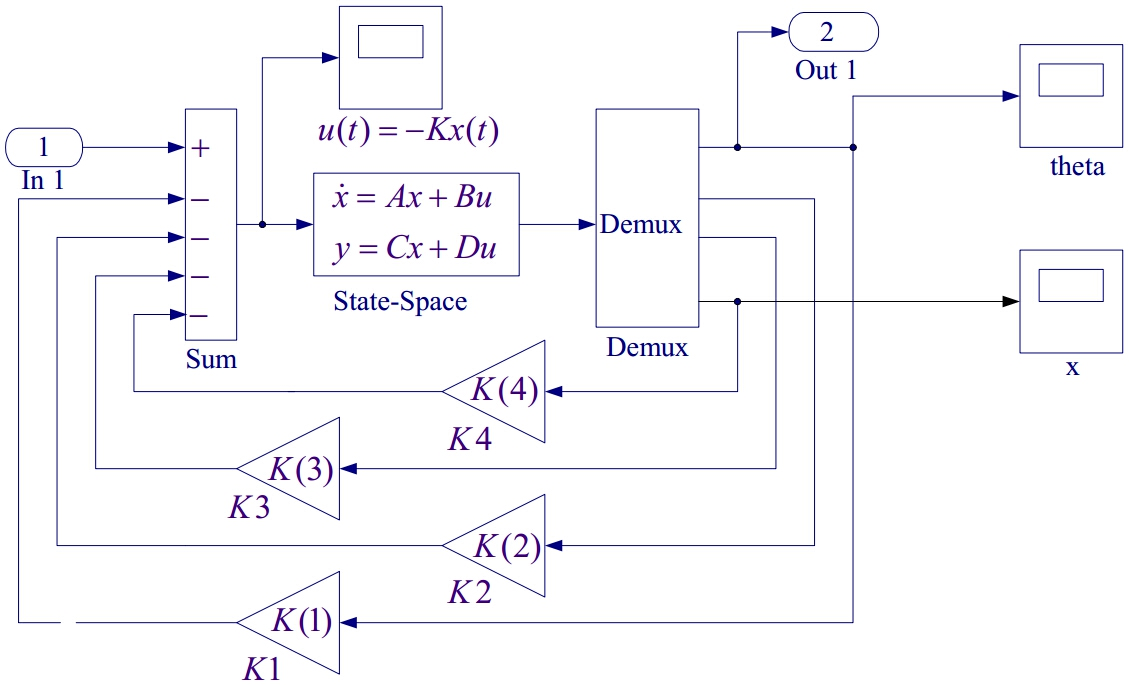
\includegraphics[width=.9\textwidth]{StateFeedbackSimulink}
\caption{\footnotesize
        Control of an inverted pendulum via pole placement.
        \label{fig.poleplacesimulink}
        }
\end{figure}

At the MATLAB prompt type the following commands to obtain the linearized transfer function model and roots of the characteristic equation:
\begin{codex}
[num, den] = linmod('Lab4CS4b');
r = roots(den);
\end{codex}
Check for the roots of the compensated system.  Are they the same as the specified values?  Is the system stable---that is---will the pendulum return to the vertical equilibrium position?

\section{Take-Home Assignment}
Experiment 4.1 and Experiment 4.2 in Cyber Exploration Laboratory at the end of Chapter 4 in \cite{nise}.

\begin{thebibliography}{9}
    \bibitem{nise} Norman Nise.  Control Systems Engineering, 6th ed.  Wiley.  2010.
    \bibitem{saadatbook} Hadi Saadat.  Computational Aids in Control Systems Using MATLAB.  McGraw-Hill.  1993.
    \bibitem{saadatsite} Hadi Saadat website. http://people.msoe.edu/~saadat/matlab.htm
\end{thebibliography}

\Closesolutionfile{ModSimSolutions}
